\subsection{Some general questions to reflect on}
\textbf{1.} Why does the mean sea level follow the shape of the Geoid?\\

\ifanswers
  \begin{tcolorbox}[enhanced jigsaw,breakable,pad at break*=1mm,
    colback=blue!5!white,colframe=babyblueeyes,title=Solutions]
  Fluids cannot sustain shear stresses. If shear stresses exist the fluid surface will adjust so that the net force is normal to the surface. Without flow the gravitational field will therefore be perpendicular to the ocean surface, which is the definition of an equipotential line. The gravitational force along that line may vary.
  \end{tcolorbox}
\fi
\textbf{2.} How can you describe the gravitational attraction between two point masses if none of them is located in the origin of the coordinate system applied?\\

\ifanswers
  \begin{tcolorbox}[enhanced jigsaw,breakable,pad at break*=1mm,
    colback=blue!5!white,colframe=babyblueeyes,title=Solutions]
    $$
      \vec{F}(\vec{r}) = -GmM \frac{1}{||\vec{r}-\vec{r_0}||^2}\frac{\vec{r}-\vec{r}_0}{||\vec{r}-\vec{r}_0||}=-GmM \frac{1}{||\vec{r}-\vec{r_0}||^3}\vec{r}-\vec{r}_0
    $$
    \begin{center}
    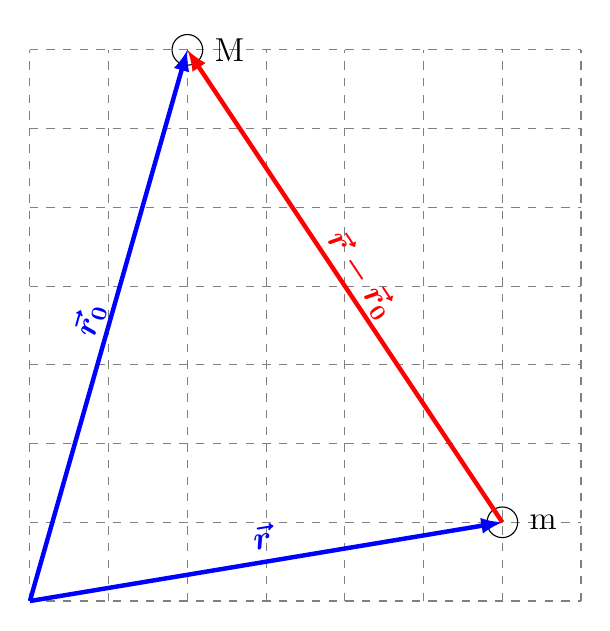
\begin{tikzpicture}[font=\boldmath]\large
      % Punkte
      \coordinate (O) at (0,0) {};
      \coordinate (A) at (6,1) {};
      \coordinate (B) at (2,7) {};
      % Draw the triangle
      % \filldraw (O) circle (3pt);
      % \filldraw (A) circle (7pt) node[sloped,midway, above] {$M$};
      % \filldraw (B) circle (3pt) node[sloped,midway, above] {$m$};
      \draw[dashed, gray] (0,0) grid (7,7);
      \node[draw,circle,label=right:m] (CircleNode) at (A)  {};
      \node[draw,circle=15pt,label=right:M] (CircleNode) at (B)  {};
      \draw[->, ultra thick, blue,   arrows={-latex}]  (O) -- (A) node[sloped,midway, above] {$\vec{r}$};
      \draw[->, ultra thick, blue,  arrows={-latex}]  (O) -- (B) node[sloped,midway,above=-0.1cm] {$\vec{r}_0$};
      \draw[->, ultra thick, red, arrows={-latex}]  (A) -- (B) node[sloped,midway,above=-0.1cm] {$\vec{r}-\vec{r}_0$};
  \end{tikzpicture}  
\end{center}
\end{tcolorbox}
\fi
\textbf{3.} How does and equipotential line change by crossing an area of (a) mass deficit, and (b) mass excess?\\

\ifanswers
  \begin{tcolorbox}[enhanced jigsaw,breakable,pad at break*=1mm,
    colback=blue!5!white,colframe=babyblueeyes,title=Solutions]
  For a mass deficit the gravitational vectors will point away from the anomaly. Therefore the corresponding equipotential lines is curved downwards. The opposite holds for a mass excess. I didn't figure out how to draw that yet in tikz.
  \end{tcolorbox}
  \fi
  \textbf{4.} Why do we have Earth \& Ocean tides? To understand the principle focus on the Moon's effect only.\\

  \ifanswers
    \begin{tcolorbox}[enhanced jigsaw,breakable,pad at break*=1mm,
      colback=blue!5!white,colframe=babyblueeyes,title=Solutions]
    It comes down to two important effects: (1) The gravitational attraction of the moon towards the Earth is strong on the near-side than on the far side due to the $r^{-2}$ dependence. This alone leads to an ellipsoidal deformation. (2) The centrifugal acceleration due to the rotation around the center of mass between Earth and Moon counterbalances this to a certain extent. The formation of tidal bulges on either side of the Earth relative to the moon can be derived by decomposing the centrifugal acceleration into a radial component and a component that is perpendicular to the rotation axis. This leads to the lunar differential gravitational field that explains tidal bulges at both sides leading to semi-diurnal tides. The sun complicates this further but does not introduce different geophysical concepts. A detailed explanation can be found in Matsuda et al. 2015 (provided on Ilias).
    \end{tcolorbox}
    \fi
    \textbf{5.} Discuss whether the sun or the moon is more important for tides.\\

  
    \ifanswers
      \begin{tcolorbox}[enhanced jigsaw,breakable,pad at break*=1mm,
        colback=blue!5!white,colframe=babyblueeyes,title=Solutions]
        The sun is much larger and has a larger potential for tidal forces, however, it is also further away. The moon on the other hand has less weight but is closer. Doing the math shows that the sun accounts for about 40\% of the tidal forces on Earth.
      \end{tcolorbox}
    \fi
      \textbf{6.} How does deglaciation support the idea of a ductile asthenosphere on top of which the continental plates 'float'? 

      \ifanswers
      \begin{tcolorbox}[enhanced jigsaw,breakable,pad at break*=1mm,
        colback=blue!5!white,colframe=babyblueeyes,title=Solutions]
        Area with strong former ice cover (e.g., Scandinavia) experience uplift today. Those uplift rates are a response to the disappearance of ice sheets, which have pushed the continents down. Now that the weight is gone, they experience isostatic uplift. This uplift does not occur instantaneously but takes many thousands of years. 
      \end{tcolorbox} 
    \fi